\documentclass[10pt,a4paper]{article}

% ---------------------------------------------------------------------------
% Chronicle -- condensed technical specification
% Compile: pdflatex chronicle-spec-condensed.tex (twice for references)
% ---------------------------------------------------------------------------

\usepackage[T1]{fontenc}
\usepackage[utf8]{inputenc}
\usepackage{lmodern}
\usepackage[margin=1.85cm,top=1.7cm,bottom=1.7cm]{geometry}
\usepackage{microtype}
\usepackage{xcolor}
\usepackage{booktabs}
\usepackage{tabularx}
\usepackage{array}
\usepackage{enumitem}
\usepackage{titlesec}
\usepackage{fancyhdr}
\usepackage{amsmath,amssymb}
\usepackage{tikz}
\usetikzlibrary{arrows.meta,positioning}
\usepackage[hidelinks]{hyperref}

\definecolor{ink}{HTML}{0F172A}
\definecolor{accent}{HTML}{0F766E}
\definecolor{accent2}{HTML}{1D4ED8}
\definecolor{muted}{HTML}{64748B}
\definecolor{panel}{HTML}{F1F5F9}
\definecolor{warn}{HTML}{B45309}

\color{ink}
\setlength{\parindent}{0pt}
\setlength{\parskip}{4pt}
\setlength{\emergencystretch}{2em}
\renewcommand{\arraystretch}{1.18}

\titleformat{\section}{\large\bfseries\color{accent}}{\thesection}{0.6em}{}
\titleformat{\subsection}{\normalsize\bfseries\color{accent2}}{\thesubsection}{0.5em}{}
\titlespacing*{\section}{0pt}{10pt}{4pt}
\titlespacing*{\subsection}{0pt}{7pt}{2pt}

\pagestyle{fancy}
\fancyhf{}
\fancyhead[L]{\footnotesize\color{muted}Chronicle --- condensed specification}
\fancyhead[R]{\footnotesize\color{muted}October 2026}
\fancyfoot[C]{\footnotesize\color{muted}\thepage}
\renewcommand{\headrulewidth}{0.2pt}
\renewcommand{\headrule}{\hbox to\headwidth{\color{panel}\leaders\hrule height \headrulewidth\hfill}}

\newcommand{\code}[1]{\texttt{\small #1}}
\newcommand{\kw}[1]{\textcolor{accent2}{\textbf{#1}}}
\newcommand{\panel}[1]{%
  \noindent\colorbox{panel}{%
    \begin{minipage}{\dimexpr\linewidth-2\fboxsep\relax}
    \vspace{1pt}#1\vspace{2pt}
    \end{minipage}}%
}

\title{\vspace{-1.2cm}\textbf{\LARGE Chronicle}\\[2pt]
\large Egocentric Episodic Memory Graph\\[2pt]
\normalsize\color{muted}Condensed technical specification --- learn it in one sitting}
\author{\normalsize Derived from the Chronicle Technical Specification and the shipped codebase}
\date{\normalsize October 2026 \quad$\cdot$\quad v1.0}

\begin{document}
\maketitle
\vspace{-0.5cm}

\begin{center}
\fcolorbox{accent!40}{panel}{\parbox{0.95\linewidth}{\small\textbf{Historical note.}
This specification describes the earlier VFM/graph prototype and its 30-question
suite. It is not the current \texttt{chronicle eval} product suite (60
deterministic checks) or the current research video results. See
\texttt{docs/README.md} for the current documentation map.}}
\end{center}

\panel{
\textbf{TL;DR.} Chronicle turns first-person video into a \emph{queryable episodic memory}, not a transcript.
It samples a video, gates heavy models behind motion and geometric events, writes a dual
(background + foreground) spatio-temporal graph to SQLite, and answers natural-language questions
from a 2-hop subgraph with timestamped citations. It runs offline with deterministic fallbacks;
a local Qwen model is an optional prose layer. A 45-second real clip's memory graph fits in
roughly \textbf{0.4\,MB}, and deterministic graph queries return in \textbf{1--5\,ms}.
}

\section{The idea in one page}

Most video assistants retrieve \emph{clips} or captions. Chronicle instead maintains
\emph{object identity over time}: where an object was, when it moved, what it rested on, and who
interacted with it. The graph is the source of truth; the language model only phrases the answer.

The pipeline is event-driven. A frame is not sent to a vision-language model unless geometry,
motion, or a state transition says something interesting happened. That single design choice is
what makes the system fast enough to feel live and small enough to keep a whole episode on disk.

\begin{center}
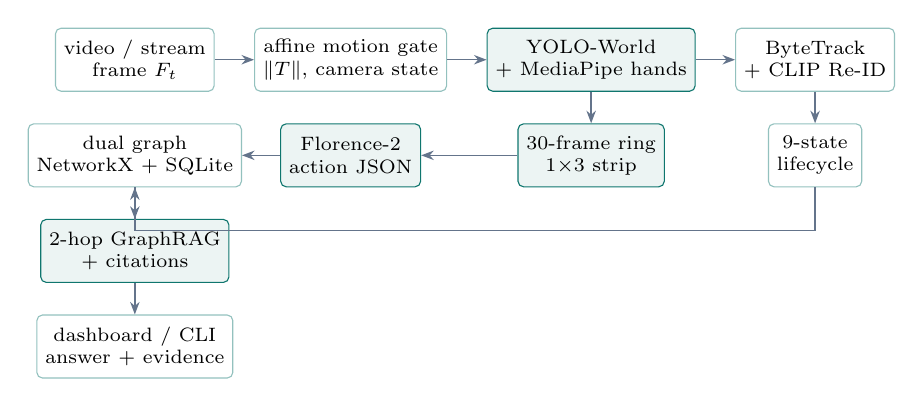
\begin{tikzpicture}[
  font=\scriptsize,
  node distance=4mm and 5mm,
  box/.style={draw=accent!45,fill=white,rounded corners=2pt,align=center,inner sep=3pt,minimum height=8mm},
  hot/.style={draw=accent,fill=accent!8,rounded corners=2pt,align=center,inner sep=3pt,minimum height=8mm},
  arr/.style={-{Stealth[length=1.6mm]},draw=muted,line width=0.5pt}
]
\node[box] (video) {video / stream\\frame $F_t$};
\node[box,right=of video] (motion) {affine motion gate\\$\lVert T\rVert$, camera state};
\node[hot,right=of motion] (det) {YOLO-World\\+ MediaPipe hands};
\node[box,right=of det] (track) {ByteTrack\\+ CLIP Re-ID};
\node[box,below=of track] (state) {9-state\\lifecycle};
\node[hot,below=of det] (clip) {30-frame ring\\1$\times$3 strip};
\node[hot,below=of motion] (vlm) {Florence-2\\action JSON};
\node[box,below=of video] (graph) {dual graph\\NetworkX + SQLite};
\node[hot,below=of graph] (rag) {2-hop GraphRAG\\+ citations};
\node[box,below=of rag] (ui) {dashboard / CLI\\answer + evidence};

\draw[arr] (video) -- (motion);
\draw[arr] (motion) -- (det);
\draw[arr] (det) -- (track);
\draw[arr] (det.south) -- (clip.north);
\draw[arr] (track.south) -- (state.north);
\draw[arr] (clip) -- (vlm);
\draw[arr] (vlm) -- (graph);
\draw[arr] (state.south) -- ++(0,-0.55) -| (graph.south);
\draw[arr] (graph) -- (rag);
\draw[arr] (rag) -- (ui);
\end{tikzpicture}
\end{center}

\textbf{Four modules, four jobs.}
\begin{itemize}[leftmargin=1.1em,itemsep=1pt,topsep=1pt]
  \item \kw{Perception}: motion gating, open-vocabulary detection, hand landmarks, tracking and Re-ID.
  \item \kw{Memory}: a 9-state lifecycle, support/containment reasoning, and a durable dual graph.
  \item \kw{Semantics}: temporal strips, Florence-2 action verification, confidence calibration, GraphRAG.
  \item \kw{Interface}: CLI, two dashboards, live ingest, uploads, snapshot/CSV export, query console.
\end{itemize}

\section{Data model: two graphs, one episode}

\begin{tabularx}{\linewidth}{@{}lX@{}}
\toprule
\textbf{Graph} & \textbf{What it stores} \\
\midrule
Background & Invariant anchors: zones (Kitchen, Work Desk) and fixed furniture (countertop, table,
sofa). Keyframes are matched by CLIP place recognition at cosine $\geq 0.85$. \\
Foreground & Episodic objects (keys, phone, mug) with persistent IDs, states, bounding boxes and
time-intervaled relations. \\
\bottomrule
\end{tabularx}

\textbf{Edges.} Spatial (\code{RESTING\_ON}, \code{INSIDE}, \code{IN\_ZONE}), temporal
(state transitions with start/end timestamps), and action multi-edges
(\code{USER --[PICKED\_UP @ t]--> KEYS}). The \emph{terminal relational anchor} is never deleted:
a long-lost object still answers ``where was it last?''.

\subsection{The 9-state lifecycle}

\begin{tabularx}{\linewidth}{@{}lX@{}}
\toprule
\textbf{State} & \textbf{Deterministic trigger (wall-clock, not frame count)} \\
\midrule
\code{NEW} & Detection with no track match and Re-ID cosine $< 0.82$. \\
\code{VISIBLE\_STATIC} & Relative velocity $\approx 0$ for $>0.5$\,s and support edge verified. \\
\code{INTERACTED} & Hand landmark containment or IoS(hand, object) $>0.60$ for $\geq 0.3$\,s. \\
\code{VISIBLE\_MOVING} & Object moves independently, hand IoS $< 0.10$. \\
\code{HELD} & Track persists, IoS $>0.50$, object centroid follows hand velocity. \\
\code{CONTAINED} & Object collapses inside a container hull, IoS $>0.85$. \\
\code{OCCLUDED} & Track lost while the camera is still and the last box overlaps an occluder. \\
\code{OUT\_OF\_VIEW} & Track lost during a camera pan; spatial anchor retained. \\
\code{LOST} & Out of view for $>600$\,s; node goes dormant, terminal anchor preserved. \\
\bottomrule
\end{tabularx}

Why this matters: the graph does not grow with frames. It grows with \emph{identity and
interaction}, and trajectories are bounded (Section 4).

\section{Perception: spend compute only where it matters}

\begin{enumerate}[leftmargin=1.1em,itemsep=1pt,topsep=1pt]
  \item \textbf{Motion gate.} Mask dynamic boxes and hands, estimate a partial affine transform
  between frames, and classify the camera as stationary or panning. Below $2.5$\,px the scene is
  still; above $8$\,px it is a pan. This separates head rotation from real object motion.
  \item \textbf{Detection.} YOLO-World is open-vocabulary but \emph{prompt-driven}: it only
  labels objects it is asked about. The starter list covers 12 objects; an opt-in broad preset
  covers 98 common indoor/egocentric objects.
  \item \textbf{Hands.} MediaPipe returns 21 landmarks. Contact is a geometric test, not a guess.
  \item \textbf{Tracking \& Re-ID.} ByteTrack supplies kinematic IDs; inactive tracks are
  re-bound by CLIP appearance similarity ($\geq 0.82$). Graph-level consolidation merges legacy
  duplicates without merging co-visible objects.
  \item \textbf{Interaction test.} Intersection over Smaller Area:
  \[
    \mathrm{IoS}(A,B)=\frac{\mathrm{Area}(A\cap B)}{\min(\mathrm{Area}(A),\mathrm{Area}(B))}
  \]
  Interaction fires when a fingertip enters the object hull, or IoS(hand, object) $>0.60$ for
  $\geq 0.3$\,s.
  \item \textbf{Temporal strip.} Keep a 30-frame RAM ring buffer. On an interaction, stitch three
  moments (pre / contact / post) into one $1\times3$ image and ask Florence-2 for an action
  caption. Strict JSON parsing and per-action thresholds reject hedged or implausible captions.
\end{enumerate}

\begin{center}
\small
\begin{tabularx}{\linewidth}{@{}lX@{}}
\toprule
\textbf{Constant} & \textbf{Value used by the implementation} \\
\midrule
Still / pan threshold & $<2.5$\,px / $>8$\,px affine magnitude \\
Re-ID cosine & $0.82$ \\
Place-recognition cosine & $0.85$ \\
Interaction / containment IoS & $0.60$ / $0.85$ \\
Interaction dwell & $0.30$\,s \\
Temporal buffer & 30 frames; strip panels $336$\,px \\
Lost / trajectory retention & $600$\,s / $600$\,s \\
Verification queue & depth 8; dedup window 1024 clips \\
Language model & \code{qwen2.5:7b-instruct}; 4096 ctx; 30\,min keep-alive \\
\bottomrule
\end{tabularx}
\end{center}

\subsection{Object appearance attributes}

Every Nth detection crop gets a cheap, deterministic appearance pass; no model
download and a few milliseconds per box on CPU.  It answers the question a label
alone cannot: \emph{which} cup?

\begin{itemize}[leftmargin=1.1em,itemsep=1pt,topsep=1pt]
  \item \textbf{Dominant colour.} Trim 10\% from every crop edge, resize the
  inner region to $\leq 64$\,px, and run $3$-means in BGR.  Cluster weights are
  a Gaussian centre prior multiplied by a background-suppression term
  $\mathrm{clip}(\lVert c-b\rVert/80,\,0.15,\,1)$, where $b$ is the median
  border colour.  The central cluster wins when it covers $\geq 12\%$ of the
  crop.  The primary BGR centroid becomes a stable colour word plus a
  \code{\#rrggbb} swatch.
  \item \textbf{Colour word.} Achromatic pixels are classified first
  ($V<42$: black; $S<35$: white/grey), then hue bands map to red, orange,
  yellow, green, cyan, blue, purple or pink.
  \item \textbf{Shape.} Bounding-box aspect ratio: $\leq 0.82$ tall,
  $\geq 1.22$ wide, otherwise square.
  \item \textbf{Size.} Relative crop area: $\leq 1.2\%$ small,
  $\leq 7.5\%$ medium, otherwise large.
  \item \textbf{Brightness / saturation.} $V<70$ dark, $V<145$ dim, else
  bright; $S<55$ muted, $S<150$ colourful, else vivid.
  \item \textbf{Texture / position.} Laplacian variance $\geq 45$ is detailed,
  else plain; the box centre gives left/centre/right and top/middle/bottom.
  \item \textbf{Stability.} A new colour replaces the track colour only when
  its confidence is at least $0.12$ higher; geometry and position update
  immediately.
\end{itemize}

The flattened attributes are persisted on the foreground entity and exposed in
snapshot/CSV exports, graph tooltips and GraphRAG.  Queries such as
\emph{``what colour is the mug?''}, \emph{``how big is it?''} and
\emph{``describe the backpack''} cite the entity's last observation with
relation \code{APPEARANCE}; a missing attribute is answered as ungrounded rather
than guessed.  The offline evaluation set includes colour, size, describe and
missing-detail cases and currently passes 13/13 with 100\% citation precision.

\section{Storage: why the graph is small}

SQLite is a durable projection of the in-memory NetworkX graph, not a second copy.
WAL mode, \code{synchronous=NORMAL}, foreign keys, and indexes keep reads
non-blocking: \code{(src, relation)}, \code{(dst, relation)},
\code{(t\_start)}, \code{(entity\_id, t\_event)}.

\begin{itemize}[leftmargin=1.1em,itemsep=1pt,topsep=1pt]
  \item \textbf{Embeddings are per identity, not per frame.} A 512-d CLIP vector is stored once
  per entity/zone as float32 (2\,KB), not for every observation.
  \item \textbf{Observations are trajectories only.} Bounding boxes and state, no pixels. Rows
  older than 10 minutes are purged. Anchors are never deleted.
  \item \textbf{Zones, furniture, transitions, edges, anchors and observations} are separate
  indexed tables; the schema is versioned in \code{meta}.
  \item \textbf{Export is portable.} \code{snapshot.json} contains graph, entities, actions,
  transitions, furniture, verification telemetry and backends; CSVs use stable headers.
\end{itemize}

\begin{center}
\small
\begin{tabularx}{\linewidth}{@{}Xrr@{}}
\toprule
\textbf{Measured on this repo (45\,s Aria kitchen clip)} & \textbf{Value} & \textbf{Unit} \\
\midrule
Source video & 2.99 & MB \\
Graph database, including WAL & 0.436 & MB \\
Entities / edges / transitions / anchors & 11 / 53 / 214 / 28 & count \\
Bounding-box observations & 536 & rows \\
Entity embeddings & 22 & KB \\
Naive per-observation 512-d embeddings & 1.05 & MB \\
Deterministic query latency & 0.14--1.05 & ms \\
Exported snapshot & 190 & KB \\
\bottomrule
\end{tabularx}
\end{center}

\textbf{Scale rule.} Storage is $O(\text{identities} + \text{interactions})$, not
$O(\text{frames})$. Trajectories are bounded by the 10-minute window; state transitions and
terminal anchors are retained. On very long videos, transitions still grow, so retention is a
policy decision, not a free lunch.

\section{Query: graph first, language second}

\begin{enumerate}[leftmargin=1.1em,itemsep=1pt,topsep=1pt]
  \item \textbf{Resolve} the entity (aliases, plurals, ambiguity-aware scoring) and the active
  zone. The result carries \code{match\_score}, \code{confidence}, \code{match\_reason} and ranked
  \code{candidates}.
  \item \textbf{Serialize} the 2-hop subgraph: latest state, spatial anchor, last interaction,
  parent zone, and the relevant action edges.
  \item \textbf{Synthesize} either a deterministic template (always available) or prose from
  local Qwen through Ollama. The model sees only the table, never the video.
  \item \textbf{Validate} every citation. A timestamp that does not map back to the subgraph is a
  hallucination and is dropped; if no valid citation remains, the answer falls back to the
  template.
\end{enumerate}

\panel{
\textbf{Example.} \emph{``Where are my keys?''} $\rightarrow$
\texttt{The keys are resting on the dining table in the kitchen [t=16.4s].}
The citation is clickable in the dashboard and seeks the video to 16.4\,s. The newest grounded
citation can also attach a supporting still frame (interaction strip, crop, zone keyframe, or an
extracted video frame).
}

\textbf{Why a small model is enough.} The hard work is retrieval and grounding. The LLM's job is
phrasing. This is also why the system survives with no model at all: the deterministic answerer
uses the same subgraph.

\section{Interfaces and operations}

\begin{center}
\begin{tabularx}{\linewidth}{@{}lX@{}}
\toprule
\textbf{Surface} & \textbf{What it is for} \\
\midrule
\code{chronicle sources} & List bundled, real and uploaded clips. \\
\code{chronicle run} & Ingest a video through perception, memory and semantics. \\
\code{chronicle ask} & Query a persisted SQLite memory from the terminal. \\
\code{chronicle serve} & Operator dashboard: live graph, timeline, tables, log, GraphRAG chat. \\
\code{run\_dashboard.py} & Mission-control dashboard: time travel, overlays, inspector, query console. \\
\code{chronicle.sh} & Start/stop/restart/status/logs/tests; LLM flags. \\
\bottomrule
\end{tabularx}
\end{center}

\begin{verbatim}
chronicle sources
chronicle run --source synthetic
chronicle ask "where are my keys?" --db data/demo/chronicle.db
chronicle serve --source synthetic --auto-run
./chronicle.sh start --llm-model qwen2.5:7b-instruct
./chronicle.sh start --no-llm
python run_dashboard.py --source demo
python -m pytest -q
\end{verbatim}

\textbf{Uploads.} Drop a clip into the operator dashboard. The targets field controls the
YOLO-World prompts (comma separated); \emph{Broad scene} enables the 98-object preset. The
chosen vocabulary is persisted in the upload's \code{source.json} manifest, and every upload gets
its own SQLite memory.

\subsection{Configuration cheat sheet}

\begin{center}
\small
\begin{tabularx}{\linewidth}{@{}lX@{}}
\toprule
\textbf{Variable} & \textbf{Default / meaning} \\
\midrule
\code{CHRONICLE\_LLM\_BACKEND} & \code{auto}, \code{ollama}, \code{transformers}, \code{template}, \code{none} \\
\code{CHRONICLE\_LLM\_MODEL} & \code{qwen2.5:7b-instruct} \\
\code{CHRONICLE\_OLLAMA\_URL} & \code{http://127.0.0.1:11434} \\
\code{CHRONICLE\_QUERY\_URL} & Optional external answer endpoint \\
\code{CHRONICLE\_DETECTOR} & \code{auto}, \code{color}, \code{yolo-world} \\
\code{CHRONICLE\_HANDS} & \code{auto}, \code{color}, \code{mediapipe} \\
\code{CHRONICLE\_EMBEDDER} & \code{auto}, \code{color}, \code{deterministic}, \code{openclip} \\
\code{CHRONICLE\_SOURCE} & \code{demo}, \code{live}, \code{jsonl}, \code{sqlite} \\
\code{CHRONICLE\_DATA\_DIR} & Asset root (default \code{./data}) \\
\bottomrule
\end{tabularx}
\end{center}

\section{Quality: what is actually verified}

\begin{itemize}[leftmargin=1.1em,itemsep=1pt,topsep=1pt]
  \item \textbf{Bounded verification queue.} Size 8, same-clip dedup, drop-oldest or reject
  policy, depth/backpressure/latency telemetry. VLM latency cannot stall ingestion.
  \item \textbf{Calibration.} Labelled captions produce per-action thresholds instead of one
  global confidence knob.
  \item \textbf{Action-timeline evaluation.} Greedy nearest-time matching against labelled
  actions; precision, recall, timestamp error, entity/container accuracy.
  \item \textbf{GraphRAG evaluation.} Location, time, action, removal, lost, zone-only and
  unknown cases; citation precision is checked per answer.
  \item \textbf{Tests.} 250+ model-free tests cover graph storage, lifecycle, query frames,
  snapshots, uploads, timeline evaluation and the dashboard smoke path.
\end{itemize}

\section{Research grounding (and what this implementation adds)}

\begin{center}
\small
\begin{tabularx}{\linewidth}{@{}lXX@{}}
\toprule
\textbf{Work} & \textbf{Idea borrowed} & \textbf{Engineering delta here} \\
\midrule
R4DSG (ACM MM 2026) & Anchor-relative 4D memory; persistent objects; no global 3D model &
Detection + tracking instead of segmentation/3D lifting; SQLite projection; 0.4\,MB per clip. \\
VL-KnG (2026) & Persistent spatio-temporal KG; graph retrieval decouples latency from video &
Millisecond deterministic queries; optional small LLM; bounded queue; no LLM-based association. \\
ESOM (WACV 2026) & Streaming object memory and online identity &
30-frame ring buffer, inactive Re-ID memory, graph consolidation; no visual query localization. \\
Hand-object contact (WACV 2024) & Contact-based interaction triggering &
Faithful IoS/hull + 0.3\,s dwell implementation with explicit JSON action validation. \\
LightMem-Ego & Working / episodic / archival tiers &
Ring buffer $\rightarrow$ foreground graph/SQLite $\rightarrow$ terminal anchors and zones. \\
\bottomrule
\end{tabularx}
\end{center}

\textbf{Honest positioning.} The research novelty is in the cited papers. Chronicle's contribution
is a compact, offline, auditable \emph{system}: small graph, fast retrieval, explicit citations,
and a UI that shows the evidence instead of asking for trust.

\section{Ten-minute demo script}

\begin{enumerate}[leftmargin=1.2em,itemsep=2pt,topsep=1pt]
  \item Start on the synthetic fixture. Show the graph, timeline and live pipeline log.
  \item Ask \emph{``Where are my keys?''} Click the citation: the video seeks to the moment.
  \item Scrub back before the placement and ask again. The answer changes. That is episodic
  memory, not a transcript.
  \item Switch to the HoloLens or Aria clip. Ask a multi-hop question:
  \emph{``Where were the keys before the drawer?''}
  \item Show the verification queue, calibration numbers and citation precision.
  \item Stop Ollama or run \code{--no-llm}; repeat a query. The deterministic answer still cites
  the graph. Robustness is part of the demo.
  \item Export \code{snapshot.json} and a CSV to show the memory is portable.
\end{enumerate}

\textbf{Pitfalls to rehearse.}
(i) YOLO-World only sees prompted labels --- use \emph{Broad scene} or name the objects.
(ii) Preload Qwen before going on stage; cold 7B load is dead air.
(iii) Checkpoint WAL before quoting database size: \code{PRAGMA wal\_checkpoint(TRUNCATE)}.
(iv) Verify evidence images exist for real clips; otherwise the frame falls back to video
extraction.
(v) Do not claim Florence-2/OpenCLIP unless those extras are installed on the demo machine.

\appendix
\section{File map}

\begin{center}
\small
\begin{tabularx}{\linewidth}{@{}lX@{}}
\toprule
\textbf{Path} & \textbf{Role} \\
\midrule
\code{chronicle/perception/} & Motion gate, detector, hands, tracker, interaction geometry. \\
\code{chronicle/graph/} & Foreground/background graphs, state machine, query engine, consolidation. \\
\code{chronicle/storage/} & SQLite schema and durable projections. \\
\code{chronicle/semantic/} & VPR, temporal strips, Florence-2, actions, queue, GraphRAG, LLM. \\
\code{chronicle/integration.py} & Runtime facade used by CLI, dashboards and demos. \\
\code{dashboard/} & Mission-control dashboard, query console, API, evidence frames. \\
\code{chronicle/ui/} & Operator dashboard (NiceGUI), uploads, snapshot import/export. \\
\code{docs/} & Contracts, role handoff notes, evaluation examples. \\
\bottomrule
\end{tabularx}
\end{center}

\section{Glossary}

\begin{description}[leftmargin=1.6em,itemsep=1pt,topsep=1pt,style=nextline]
  \item[IoS] Intersection over Smaller Area; containment-friendly alternative to IoU.
  \item[VPR] Visual place recognition; CLIP keyframe matching for zone relocalization.
  \item[Re-ID] Re-identification; appearance matching that re-binds a lost track to an entity.
  \item[Terminal anchor] The last verified spatial relation of an object; never deleted.
  \item[GraphRAG] Retrieve a 2-hop subgraph, then synthesize a grounded answer.
  \item[Evidence frame] The still image that supports an answer: interaction strip, crop,
  zone keyframe, or extracted video frame.
\end{description}

\end{document}
